\documentclass[a4paper]{extarticle}

% \usepackage[T1]{fontenc}
\usepackage[utf8]{inputenc}
\usepackage[english]{babel}
\usepackage{natbib}

\usepackage{geometry}

\usepackage{subcaption}
\usepackage[mathcal]{euscript}

\usepackage{graphicx, url}

\usepackage{amsmath, amsfonts, amssymb, amsthm}
\usepackage{mathptmx}

\usepackage{grffile}

\graphicspath{{../assets/}}

\title{Bayesian Sparsification of Deep $\cplx$-valued networks -- Extended appendix}
\author{Ivan Nazarov, and Evgeny Burnaev}

%% notation
\newcommand{\real}{\mathbb{R}}
\newcommand{\cplx}{\mathbb{C}}
\newcommand{\tr}[1]{\mathop{tr}{#1}}

\newcommand{\hop}{{\mkern-1.5mu\dagger}}
\newcommand{\conj}[1]{\overline{#1}}

% \renewcommand{\top}{{\mkern-1.5mu\intercal}}
\renewcommand{\vec}[1]{\overrightarrow{#1}}
\newcommand{\diag}[1]{\mathrm{diag}{#1}}

\begin{document}
\maketitle
\tableofcontents
\listoffigures
\clearpage

\section{MNIST-like experiments} % (fold)
\label{sec:mnist_like_experiments}

To supplement the results, reported in the main text (figures \ref{fig:paper__mnist-like__trade-off__VD__fft}
and \ref{fig:paper__mnist-like__trade-off__VD__raw}), we conduct additional experiments
with the same basic set-up, but over a finer grid of KL-divergence term coefficients.
%
These experiments lend further evidence in support of the conclusions, drawn in the main
paper, namely, that the $\cplx$-valued extension of the $\real$-valued variational dropout
can offer significant compression levels without much loss in performance. At the same
time, the test performance of both $\real$ and $\cplx$ compressed networks benefits from
an extra fine-tuning stage, during which sparsity masks are fixed.

One intriguing observation, is that on MNIST-like images the dense network, taking Fourier
features on input, exhibits gradually improving test-split performance. This is in stark
contrast to raw image input, where the performance stays at one level in the small compression
regime, and then gradually decays at high compression levels. Noteworthy is the presence
of a trough in the pre fine-tuning stage performance in the small compression regime on figures
\ref{fig:appendix__mnist-like__trade-off__ARD__raw},
\ref{fig:appendix__mnist-like__trade-off__VD__raw},
\ref{fig:appendix__cmp__mnist-like__trade-off__ARD__raw},
and \ref{fig:appendix__cmp__mnist-like__trade-off__VD__raw}, which then slowly disappears
as compression increases.

The following scatter plots depict the samples from the compression-performance trade-off
curve of simple networks studied in the experiments on the MNIST-like datasets. Transparent
horizontal bands on each plot represent min-max performance spread of an uncompressed
network on the test split. The points illustrate the final trade-off of the compressed
networks after fine-tuning, while their tails show the performance gain or loss due to
the fine-tuning.

We recap the set-up of each additional experiment on MNIST-like datasets:
\begin{itemize}
  \item staged training, with weight and optimizer state transfer
  \item $40$, $75$, and $40$ epochs for ``dense'', ``sparsify'', and ``fine-tune'' stagers, respectively
  \item ADAM optimizer with learning rate $10^{-3}$ before the $10$-th, and $10^{-4}$
  afterwards
  \item global $\ell_2$-norm gradient clipping set at $\tfrac12$
  \item training batches of size $128$ from a fixed randomly subset ($10^4$ images) of the training split
  \item the multiplier of the Kullback-Leibler term in ELBO varies over $
    C \in \{
      \tfrac32 2^{-\tfrac{k}2} \colon k=2, \cdots, 38
    \}
  $
  \item the sparsification threshold $\tau$ is set to $-\tfrac12$
\end{itemize}
Each experiment has been performed $5$ times to obtain a small sample of performance-compression
values for each setting of $C$. By reevaluating each setting several times we can account
for randomness in initialization of the uncompressed network at ``dense'', stochasticity of
variational dropout layers, randomness of batch sequences during SDG, and non-determinism
of computations on GPUs.

Each figure shows the compression-accuracy trade-off of a particular method and input features
for \textit{SimpleConvModel} and \textit{TwoLayerDenseModel} models for all four of the studied
datasets (described in the main text): \emph{top-left} EMNIST-Letters, \emph{top-right} KMNIST,
\emph{bottom-left} Fashion MNIST, and \emph{bottom-right} MNIST.
%
Figures \ref{fig:appendix__mnist-like__trade-off__ARD__fft}, \ref{fig:appendix__mnist-like__trade-off__VD__fft},
\ref{fig:appendix__mnist-like__trade-off__ARD__raw}, and \ref{fig:appendix__mnist-like__trade-off__VD__raw}
present $\real$ and $\cplx$ models with \emph{the same architecture}. We also report the
trade-off comparison, when the argument by \citet{monning_evaluation_2018} for higher intrinsic
capacity of $\cplx$-valued networks has been taken into account.
%
We compare $\real$ networks against $\tfrac12 \cplx$ with half the number of parameters
for raw input features on figures \ref{fig:appendix__cmp__mnist-like__trade-off__ARD__raw},
and \ref{fig:appendix__cmp__mnist-like__trade-off__VD__raw}, and $2 \real$ with
double the number of parameters against $\cplx$ for Fourier input features on figures
\ref{fig:appendix__cmp__mnist-like__trade-off__ARD__fft} and
\ref{fig:appendix__cmp__mnist-like__trade-off__VD__fft}.

The following observations can be made from the conducted experiment:
\begin{itemize}
  \item $\cplx$-valued networks do not have as much spare capacity as $2 \real$ due to
  constants imposed by multiplication in $\cplx$ numbers (\ref{fig:appendix__cmp__mnist-like__trade-off__ARD__raw},
  \ref{fig:appendix__cmp__mnist-like__trade-off__VD__raw})
  \item Variational Dropout and Automatic Relevance Determination offer similar compression-performance
  trade-off, with negligibly lower compression by the latter (both $\real$ and $\cplx$ versions,
  e.g. figures \ref{fig:appendix__mnist-like__trade-off__ARD__raw} and \ref{fig:appendix__mnist-like__trade-off__VD__raw})
  \item smaller networks tend to be less compressible (figures \ref{fig:appendix__cmp__mnist-like__trade-off__ARD__fft},
  \ref{fig:appendix__cmp__mnist-like__trade-off__VD__fft})
\end{itemize}

\begin{figure}[b]
  \centering
  \begin{subfigure}[b]{0.5\textwidth}
    \centering
    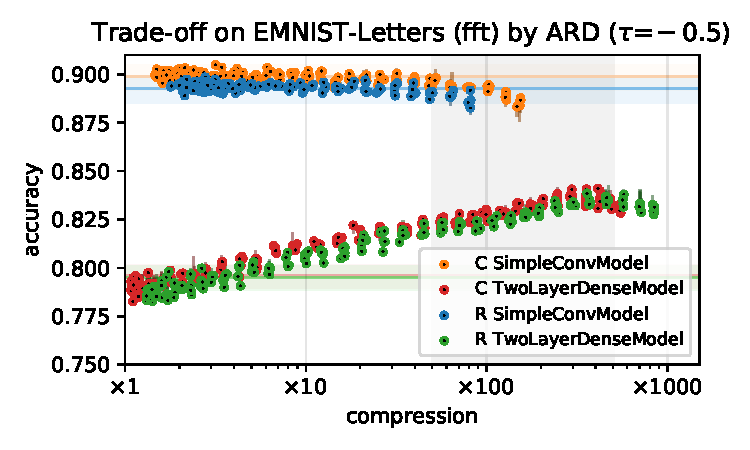
\includegraphics[width=\linewidth]{figure__mnist-like__trade-off/appendix__ARD__emnist_letters__fft__-0.5.pdf}
  \end{subfigure}%
  \begin{subfigure}[b]{0.5\textwidth}
    \centering
    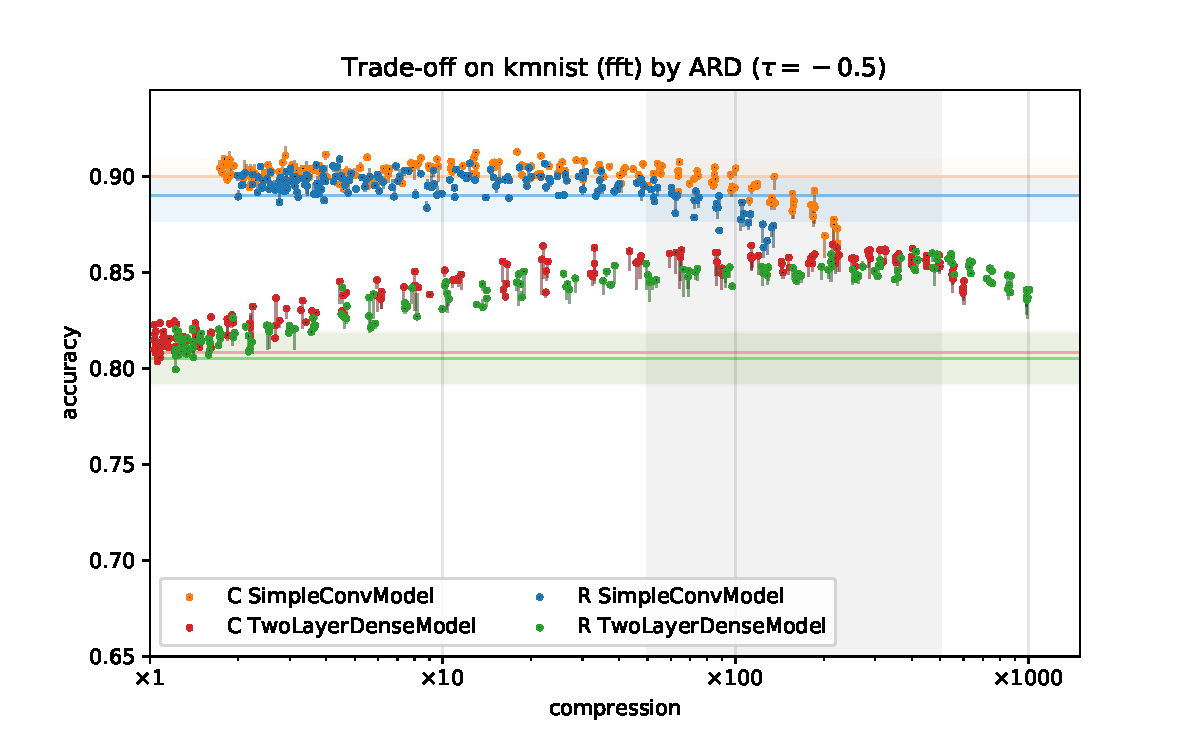
\includegraphics[width=\linewidth]{figure__mnist-like__trade-off/appendix__ARD__kmnist__fft__-0.5.pdf}
  \end{subfigure} \\ %
  \begin{subfigure}[b]{0.5\textwidth}
    \centering
    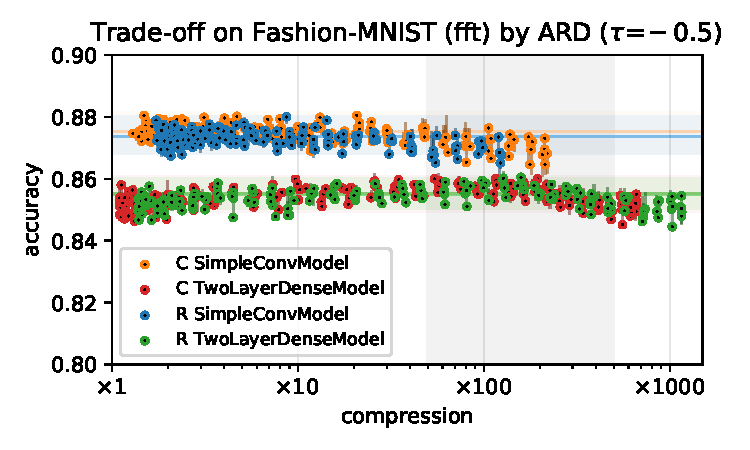
\includegraphics[width=\linewidth]{figure__mnist-like__trade-off/appendix__ARD__fashionmnist__fft__-0.5.pdf}
  \end{subfigure}%
  \begin{subfigure}[b]{0.5\textwidth}
    \centering
    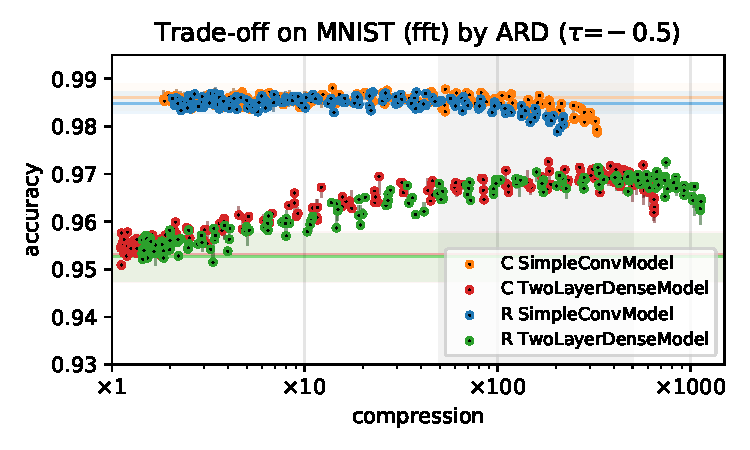
\includegraphics[width=\linewidth]{figure__mnist-like__trade-off/appendix__ARD__mnist__fft__-0.5.pdf}
  \end{subfigure}
  \caption{%
    The trade-off of ARD method for $\real$ and $\cplx$ models using Fourier features.
  }
  \label{fig:appendix__mnist-like__trade-off__ARD__fft}
\end{figure}

\begin{figure}[b]
  \centering
  \begin{subfigure}[b]{0.5\textwidth}
    \centering
    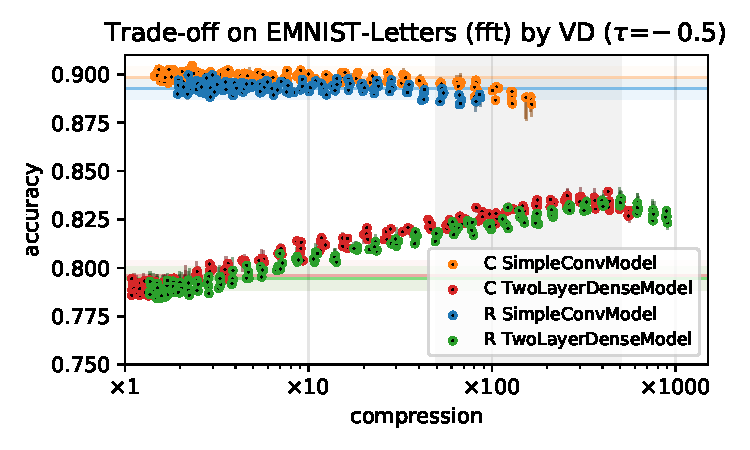
\includegraphics[width=\linewidth]{figure__mnist-like__trade-off/appendix__VD__emnist_letters__fft__-0.5.pdf}
  \end{subfigure}%
  \begin{subfigure}[b]{0.5\textwidth}
    \centering
    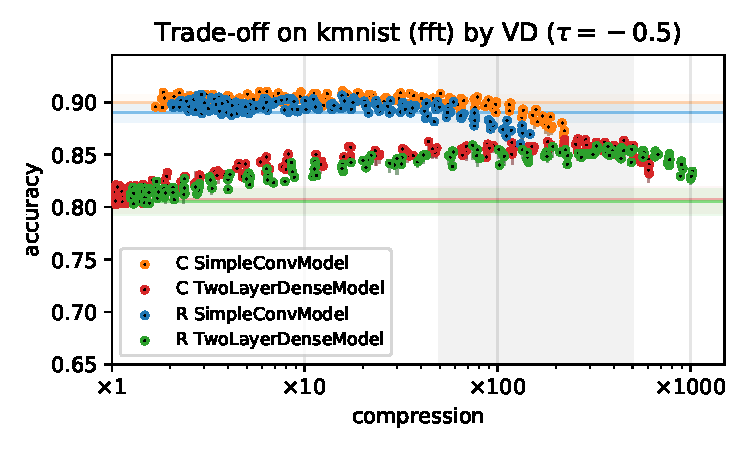
\includegraphics[width=\linewidth]{figure__mnist-like__trade-off/appendix__VD__kmnist__fft__-0.5.pdf}
  \end{subfigure} \\ %
  \begin{subfigure}[b]{0.5\textwidth}
    \centering
    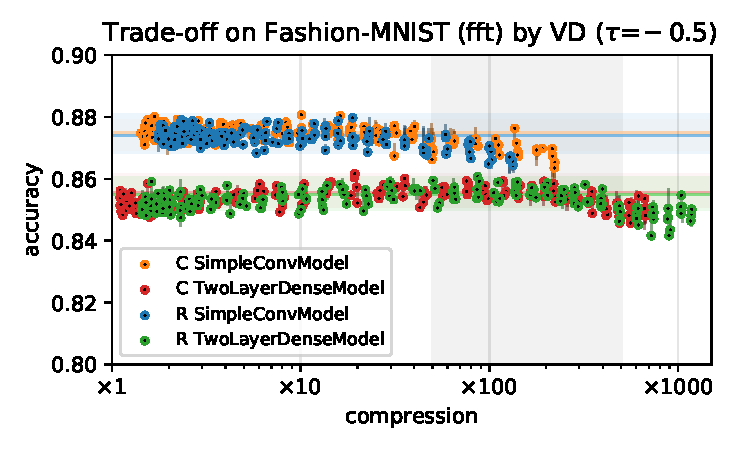
\includegraphics[width=\linewidth]{figure__mnist-like__trade-off/appendix__VD__fashionmnist__fft__-0.5.pdf}
  \end{subfigure}%
  \begin{subfigure}[b]{0.5\textwidth}
    \centering
    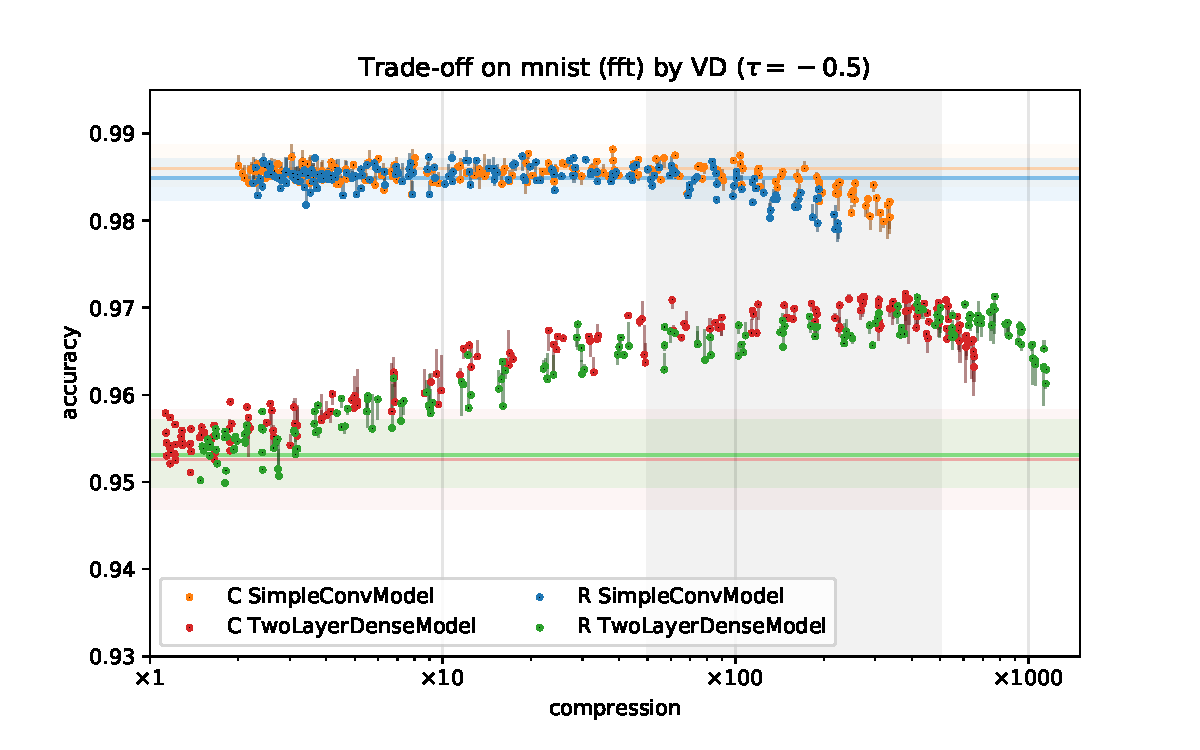
\includegraphics[width=\linewidth]{figure__mnist-like__trade-off/appendix__VD__mnist__fft__-0.5.pdf}
  \end{subfigure}
  \caption{%
    The trade-off of VD method for $\real$ and $\cplx$ models using Fourier features.
  }
  \label{fig:appendix__mnist-like__trade-off__VD__fft}
\end{figure}

\begin{figure}[b]
  \centering
  \begin{subfigure}[b]{0.5\textwidth}
    \centering
    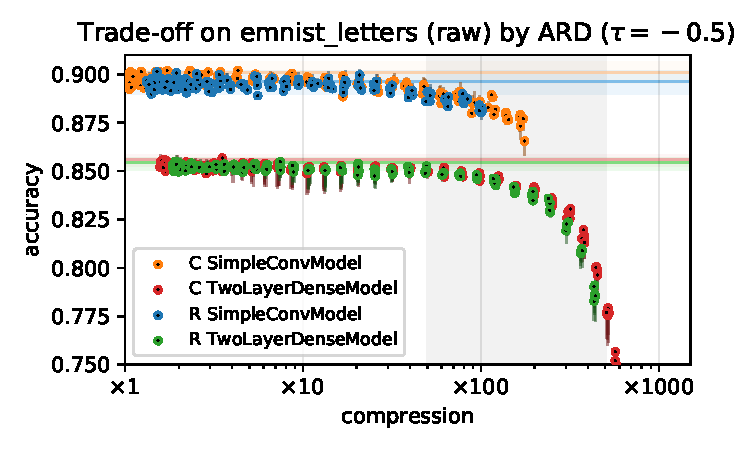
\includegraphics[width=\linewidth]{figure__mnist-like__trade-off/appendix__ARD__emnist_letters__raw__-0.5.pdf}
  \end{subfigure}%
  \begin{subfigure}[b]{0.5\textwidth}
    \centering
    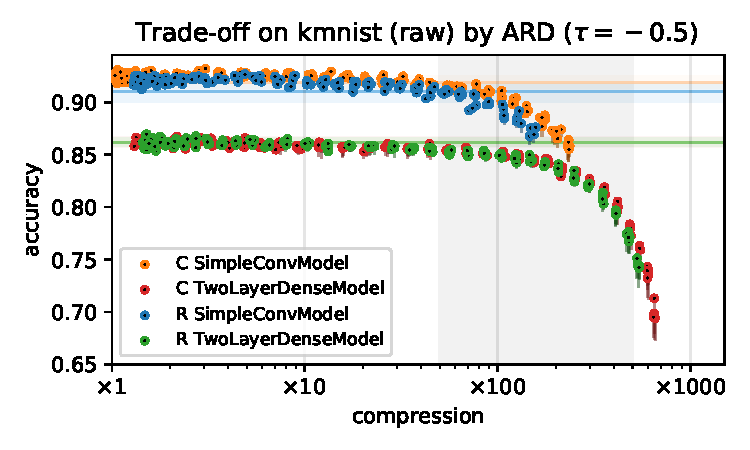
\includegraphics[width=\linewidth]{figure__mnist-like__trade-off/appendix__ARD__kmnist__raw__-0.5.pdf}
  \end{subfigure} \\%
  \begin{subfigure}[b]{0.5\textwidth}
    \centering
    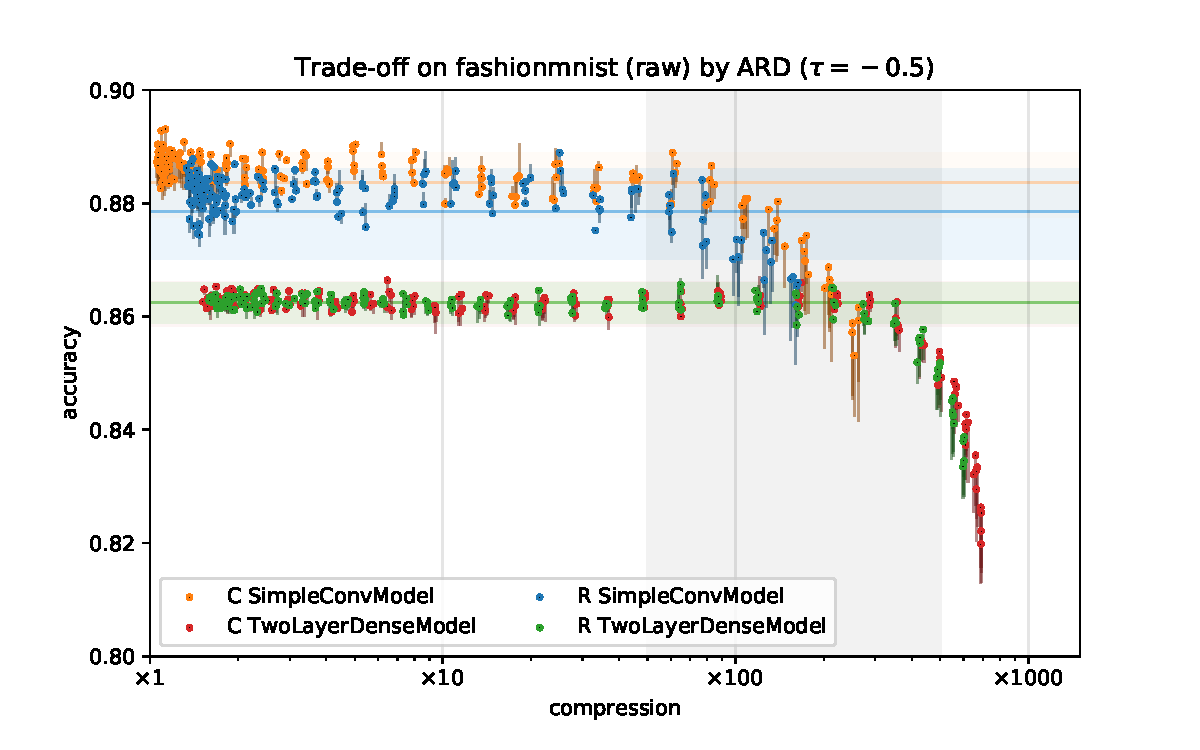
\includegraphics[width=\linewidth]{figure__mnist-like__trade-off/appendix__ARD__fashionmnist__raw__-0.5.pdf}
  \end{subfigure}%
  \begin{subfigure}[b]{0.5\textwidth}
    \centering
    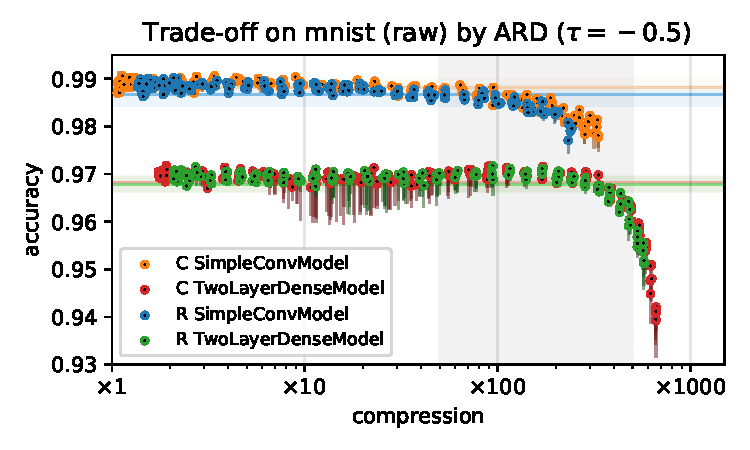
\includegraphics[width=\linewidth]{figure__mnist-like__trade-off/appendix__ARD__mnist__raw__-0.5.pdf}
  \end{subfigure}
  \caption{%
    The trade-off of ARD method for $\real$ and $\cplx$ models using raw features.
  }
  \label{fig:appendix__mnist-like__trade-off__ARD__raw}
\end{figure}

\begin{figure}[b]
  \centering
  \begin{subfigure}[b]{0.5\textwidth}
    \centering
    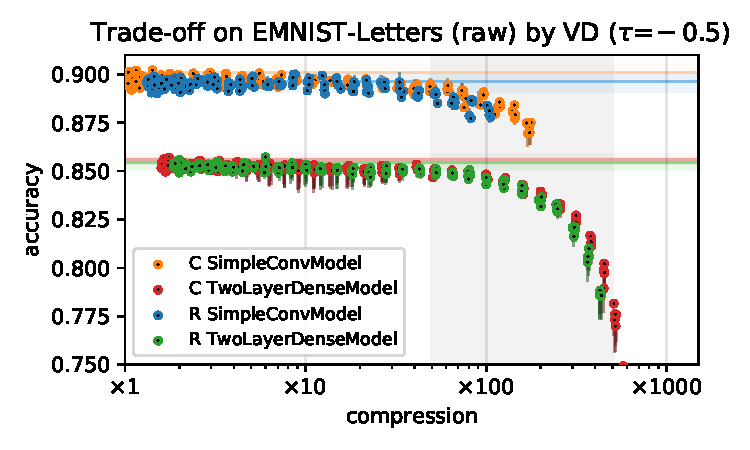
\includegraphics[width=\linewidth]{figure__mnist-like__trade-off/appendix__VD__emnist_letters__raw__-0.5.pdf}
  \end{subfigure}%
  \begin{subfigure}[b]{0.5\textwidth}
    \centering
    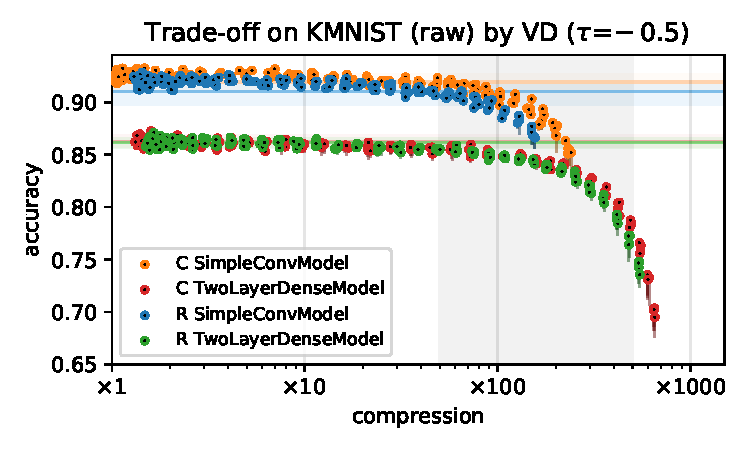
\includegraphics[width=\linewidth]{figure__mnist-like__trade-off/appendix__VD__kmnist__raw__-0.5.pdf}
  \end{subfigure} \\%
  \begin{subfigure}[b]{0.5\textwidth}
    \centering
    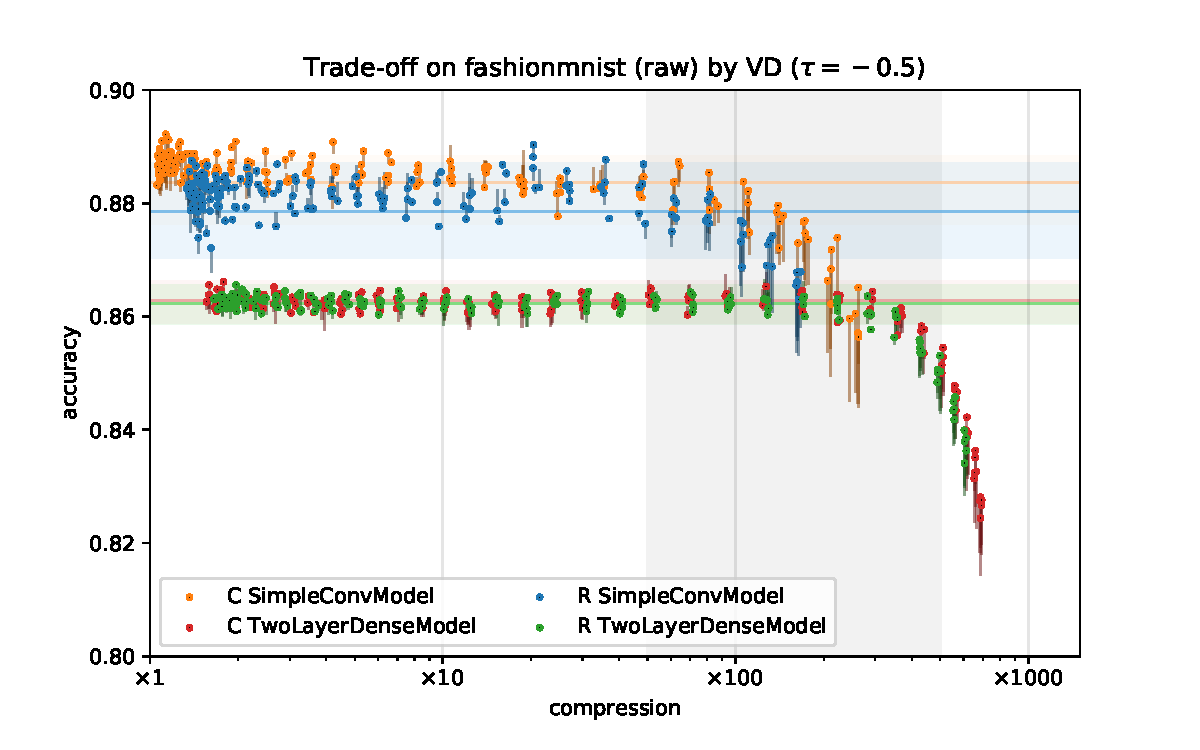
\includegraphics[width=\linewidth]{figure__mnist-like__trade-off/appendix__VD__fashionmnist__raw__-0.5.pdf}
  \end{subfigure}%
  \begin{subfigure}[b]{0.5\textwidth}
    \centering
    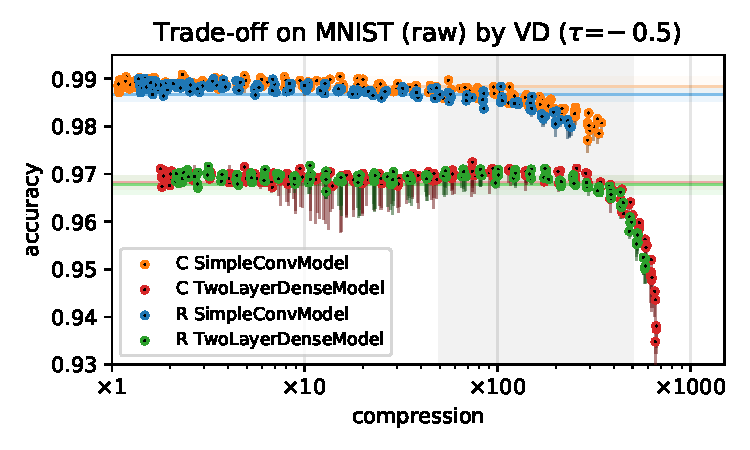
\includegraphics[width=\linewidth]{figure__mnist-like__trade-off/appendix__VD__mnist__raw__-0.5.pdf}
  \end{subfigure}
  \caption{%
    The trade-off of VD method for $\real$ and $\cplx$ models using raw features.
  }
  \label{fig:appendix__mnist-like__trade-off__VD__raw}
\end{figure}

\begin{figure}[b]
  \centering
  \begin{subfigure}[b]{0.5\textwidth}
    \centering
    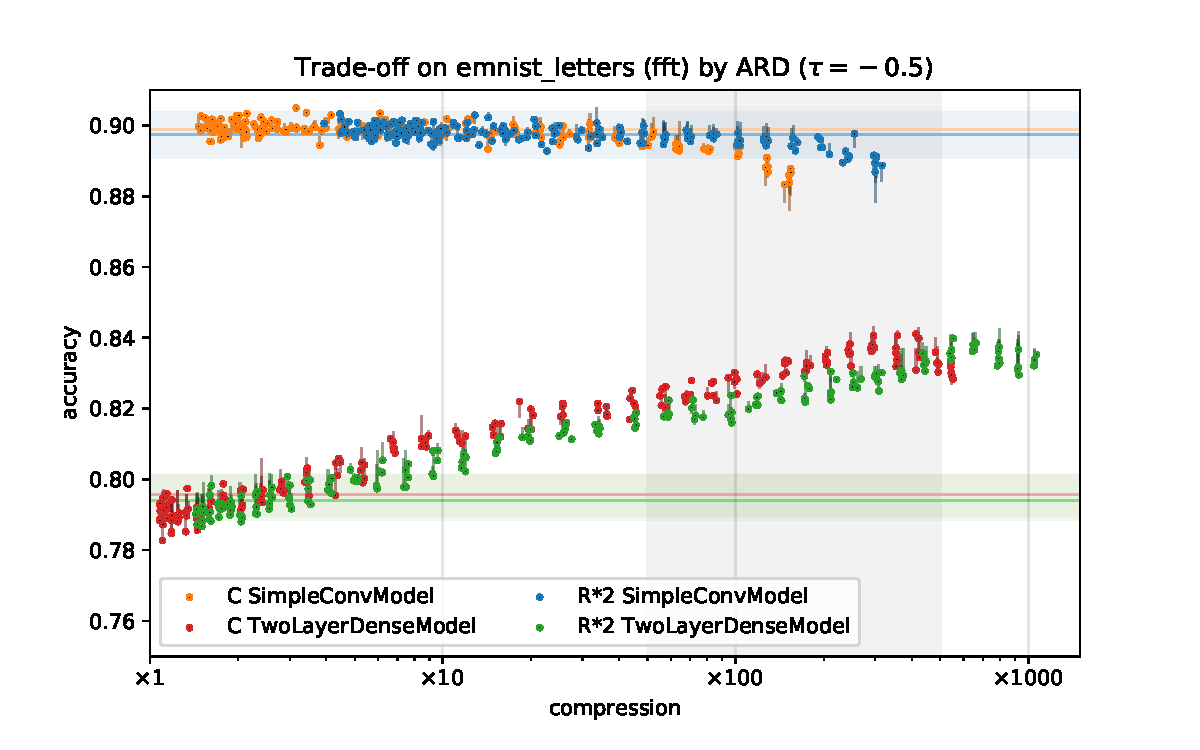
\includegraphics[width=\linewidth]{figure__mnist-like__trade-off/appendix__cmp__ARD__emnist_letters__fft__-0.5.pdf}
  \end{subfigure}%
  \begin{subfigure}[b]{0.5\textwidth}
    \centering
    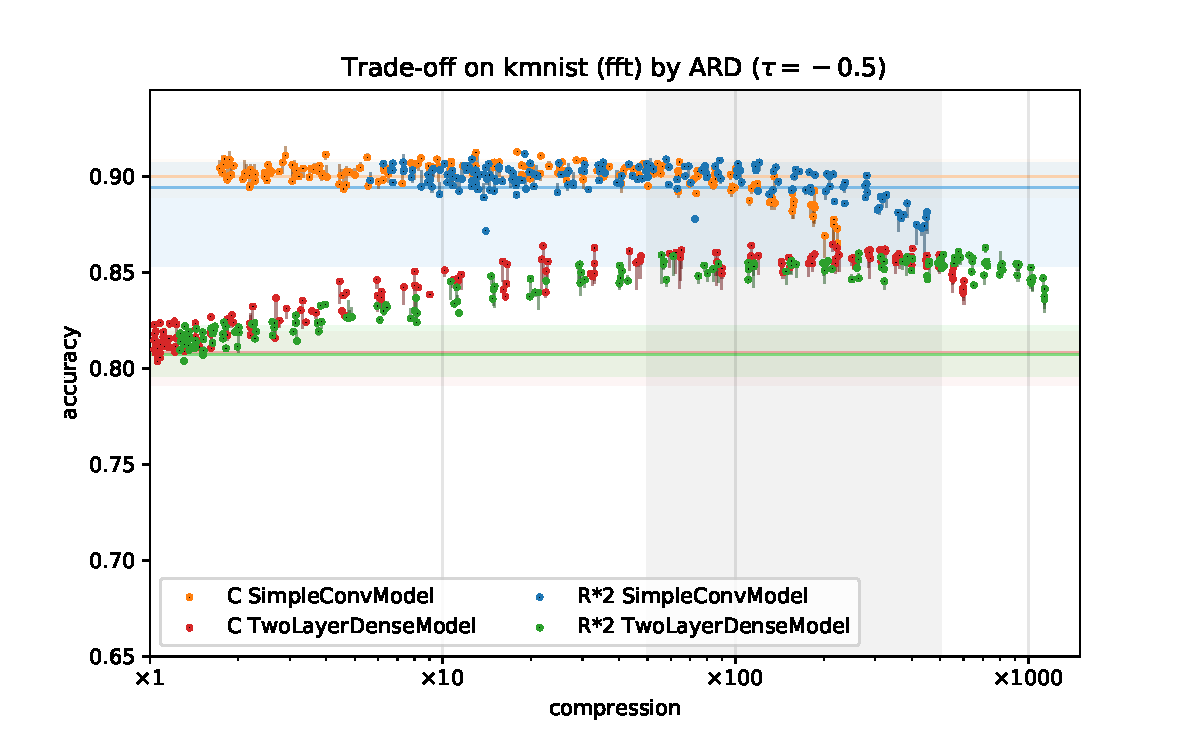
\includegraphics[width=\linewidth]{figure__mnist-like__trade-off/appendix__cmp__ARD__kmnist__fft__-0.5.pdf}
  \end{subfigure} \\ %
  \begin{subfigure}[b]{0.5\textwidth}
    \centering
    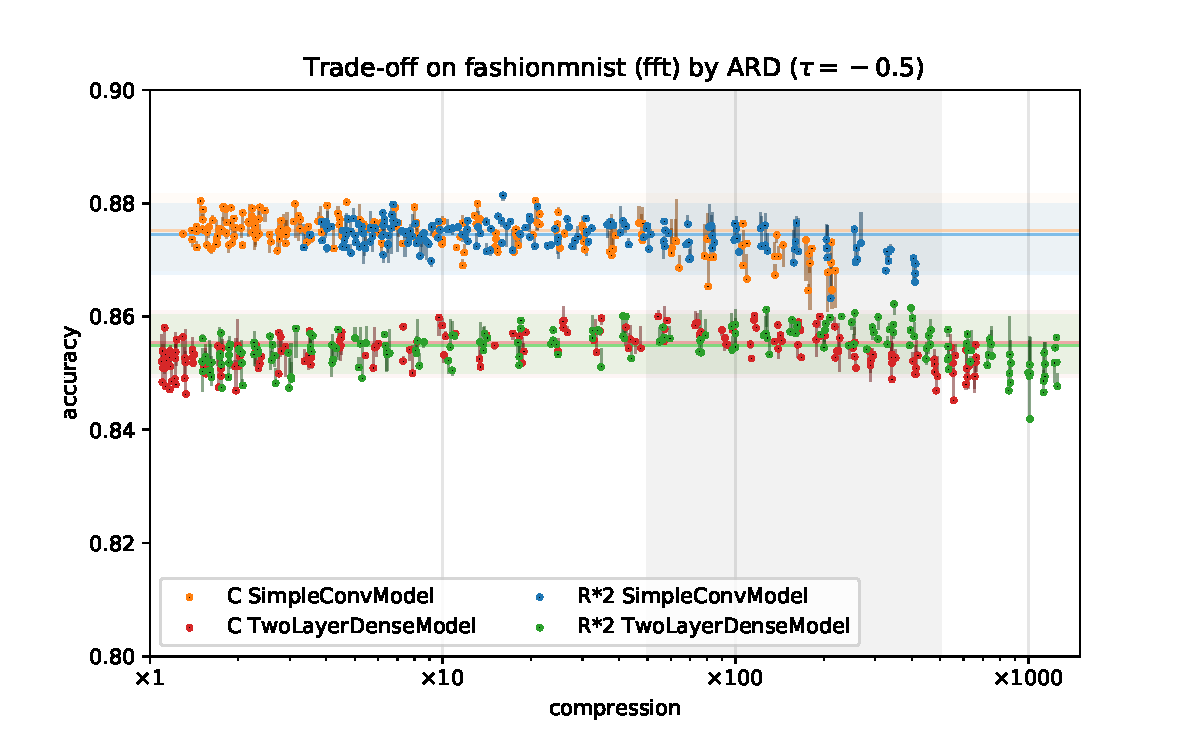
\includegraphics[width=\linewidth]{figure__mnist-like__trade-off/appendix__cmp__ARD__fashionmnist__fft__-0.5.pdf}
  \end{subfigure}%
  \begin{subfigure}[b]{0.5\textwidth}
    \centering
    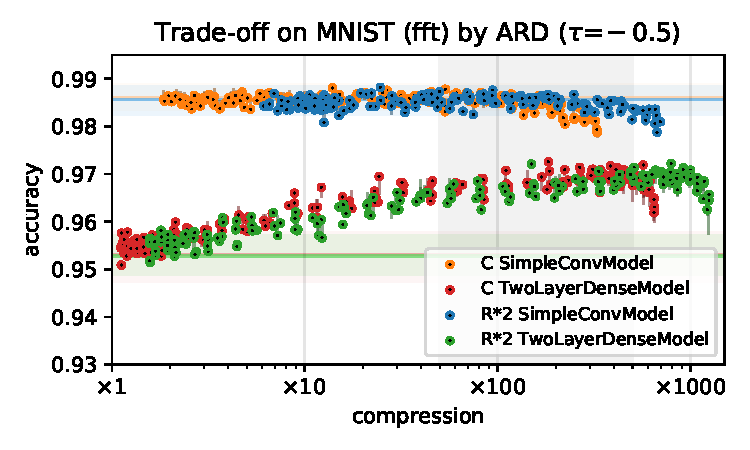
\includegraphics[width=\linewidth]{figure__mnist-like__trade-off/appendix__cmp__ARD__mnist__fft__-0.5.pdf}
  \end{subfigure}
  \caption{%
    The trade-off of ARD method for $2\real$ and $\cplx$ models using Fourier features.
  }
  \label{fig:appendix__cmp__mnist-like__trade-off__ARD__fft}
\end{figure}

\begin{figure}[b]
  \centering
  \begin{subfigure}[b]{0.5\textwidth}
    \centering
    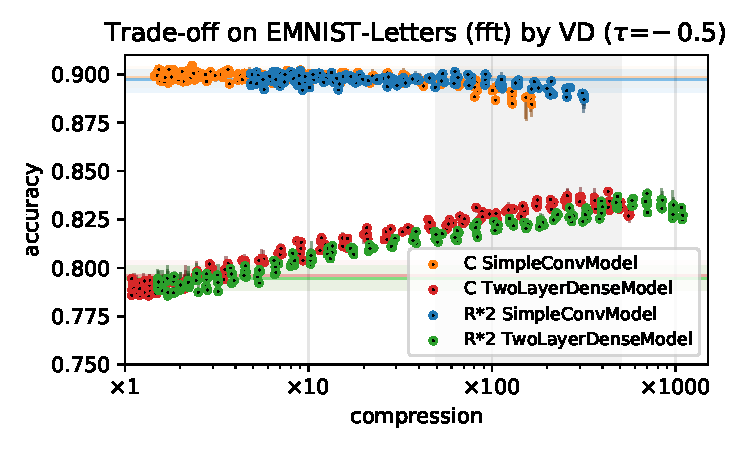
\includegraphics[width=\linewidth]{figure__mnist-like__trade-off/appendix__cmp__VD__emnist_letters__fft__-0.5.pdf}
  \end{subfigure}%
  \begin{subfigure}[b]{0.5\textwidth}
    \centering
    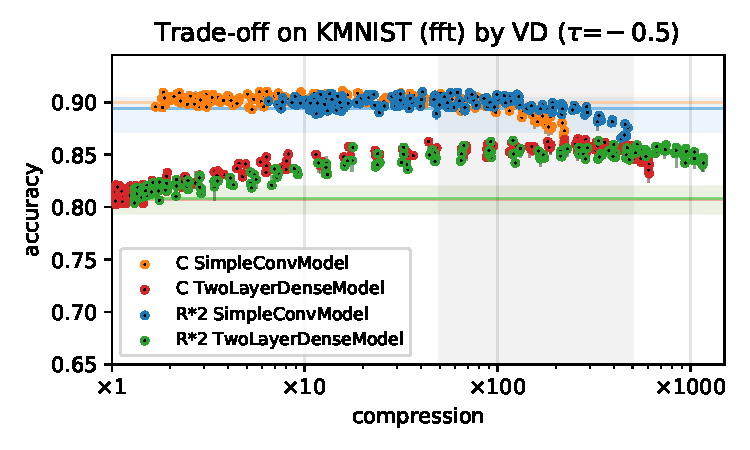
\includegraphics[width=\linewidth]{figure__mnist-like__trade-off/appendix__cmp__VD__kmnist__fft__-0.5.pdf}
  \end{subfigure} \\ %
  \begin{subfigure}[b]{0.5\textwidth}
    \centering
    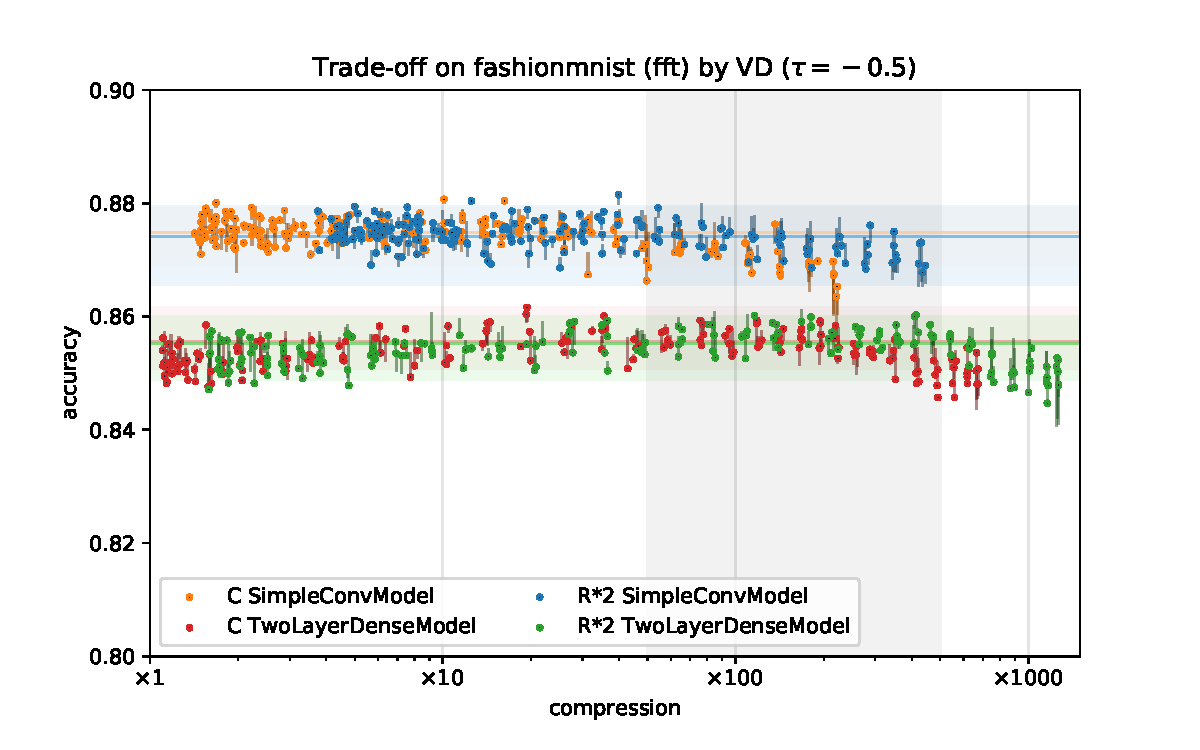
\includegraphics[width=\linewidth]{figure__mnist-like__trade-off/appendix__cmp__VD__fashionmnist__fft__-0.5.pdf}
  \end{subfigure}%
  \begin{subfigure}[b]{0.5\textwidth}
    \centering
    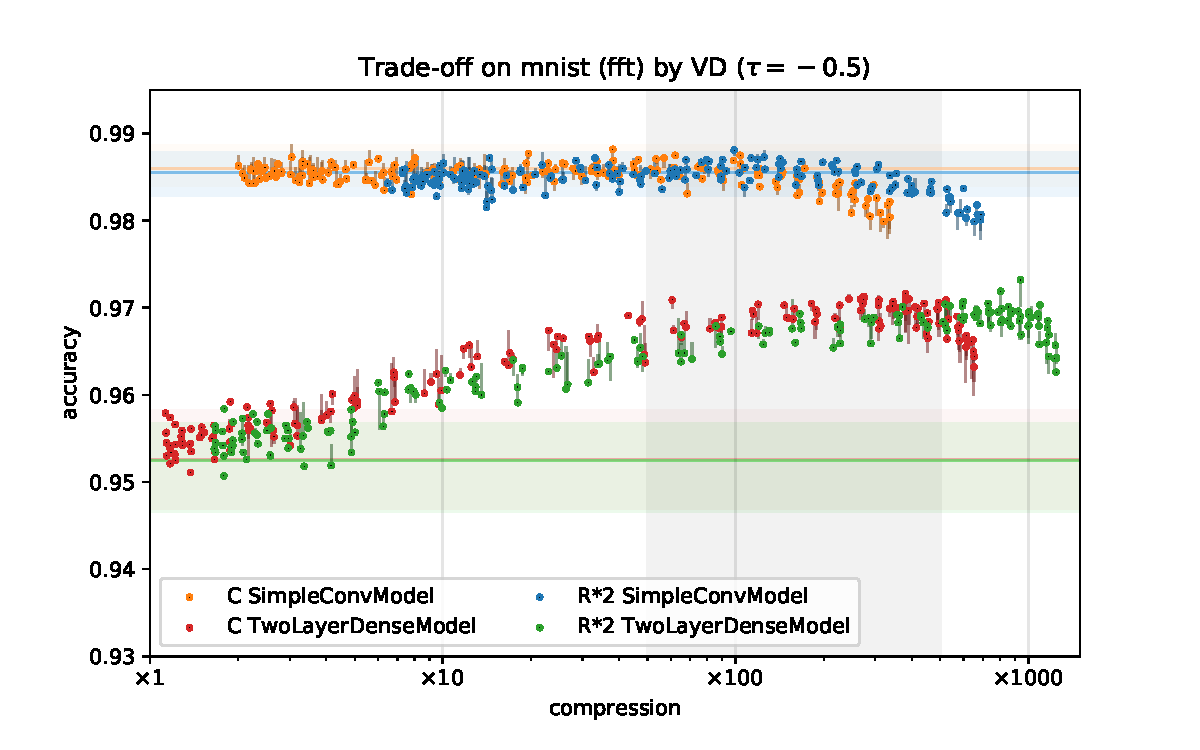
\includegraphics[width=\linewidth]{figure__mnist-like__trade-off/appendix__cmp__VD__mnist__fft__-0.5.pdf}
  \end{subfigure}
  \caption{%
    The trade-off of VD method for $2\real$ and $\cplx$ models using Fourier features.
  }
  \label{fig:appendix__cmp__mnist-like__trade-off__VD__fft}
\end{figure}

\begin{figure}[b]
  \centering
  \begin{subfigure}[b]{0.5\textwidth}
    \centering
    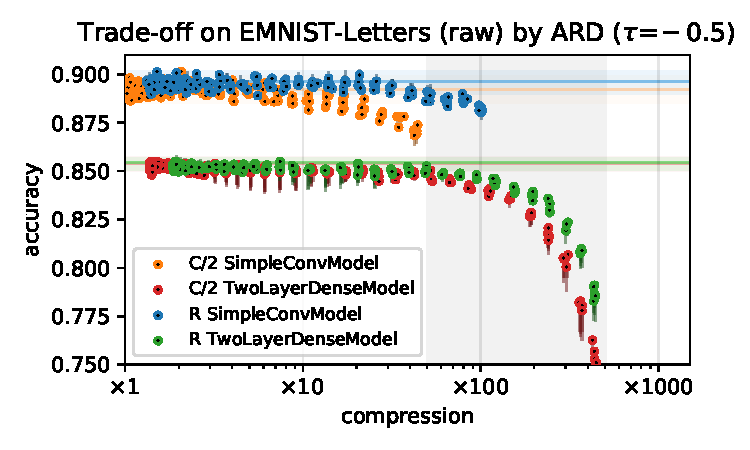
\includegraphics[width=\linewidth]{figure__mnist-like__trade-off/appendix__cmp__ARD__emnist_letters__raw__-0.5.pdf}
  \end{subfigure}%
  \begin{subfigure}[b]{0.5\textwidth}
    \centering
    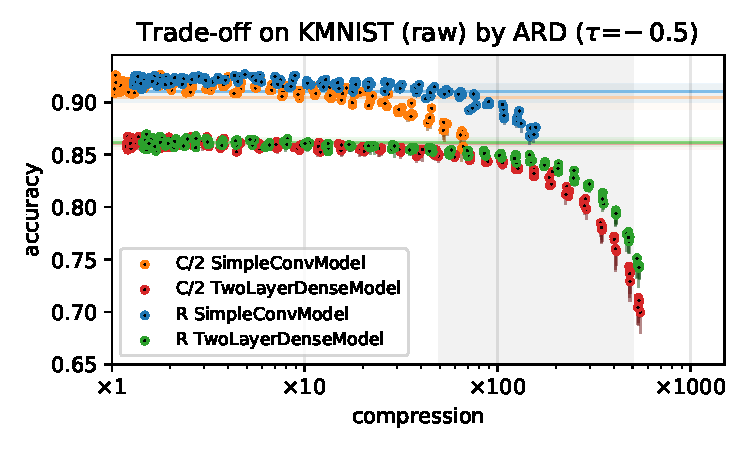
\includegraphics[width=\linewidth]{figure__mnist-like__trade-off/appendix__cmp__ARD__kmnist__raw__-0.5.pdf}
  \end{subfigure} \\%
  \begin{subfigure}[b]{0.5\textwidth}
    \centering
    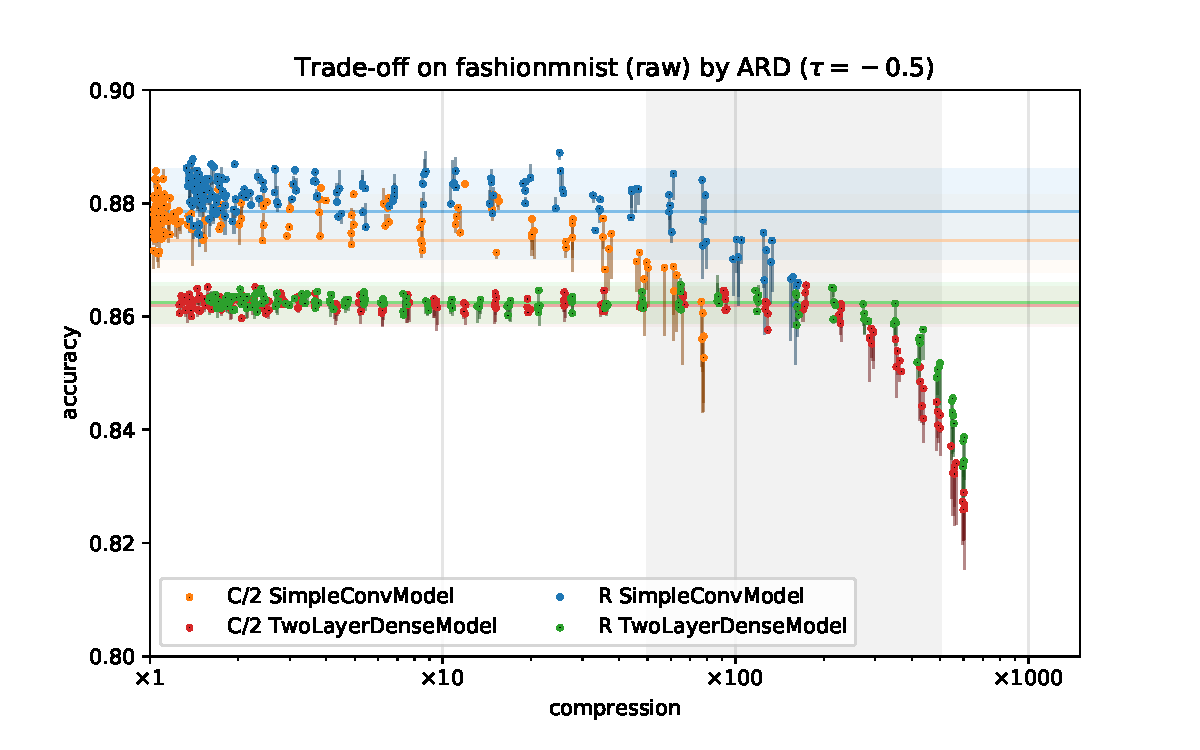
\includegraphics[width=\linewidth]{figure__mnist-like__trade-off/appendix__cmp__ARD__fashionmnist__raw__-0.5.pdf}
  \end{subfigure}%
  \begin{subfigure}[b]{0.5\textwidth}
    \centering
    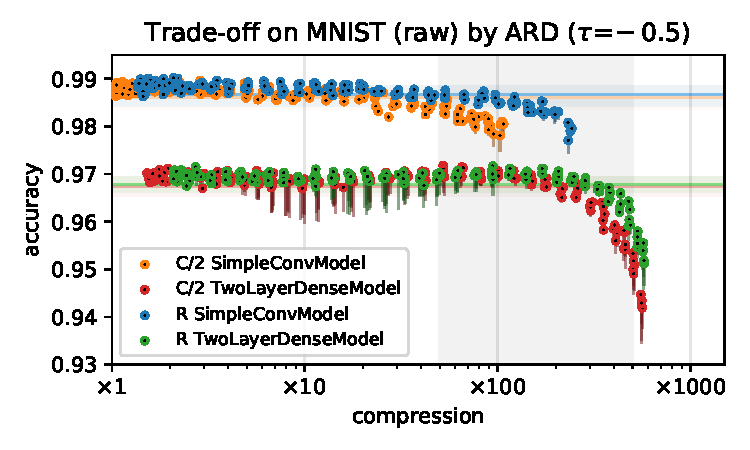
\includegraphics[width=\linewidth]{figure__mnist-like__trade-off/appendix__cmp__ARD__mnist__raw__-0.5.pdf}
  \end{subfigure}
  \caption{%
    The trade-off of ARD method for $\real$ and $\tfrac12\cplx$ models using raw features.
  }
  \label{fig:appendix__cmp__mnist-like__trade-off__ARD__raw}
\end{figure}

\begin{figure}[b]
  \centering
  \begin{subfigure}[b]{0.5\textwidth}
    \centering
    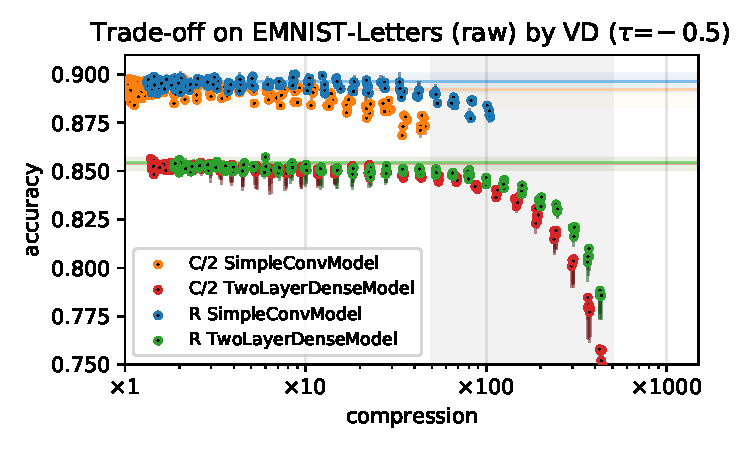
\includegraphics[width=\linewidth]{figure__mnist-like__trade-off/appendix__cmp__VD__emnist_letters__raw__-0.5.pdf}
  \end{subfigure}%
  \begin{subfigure}[b]{0.5\textwidth}
    \centering
    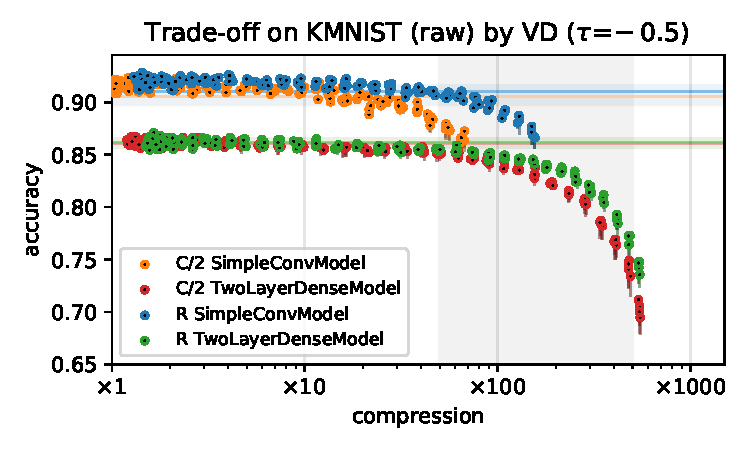
\includegraphics[width=\linewidth]{figure__mnist-like__trade-off/appendix__cmp__VD__kmnist__raw__-0.5.pdf}
  \end{subfigure} \\%
  \begin{subfigure}[b]{0.5\textwidth}
    \centering
    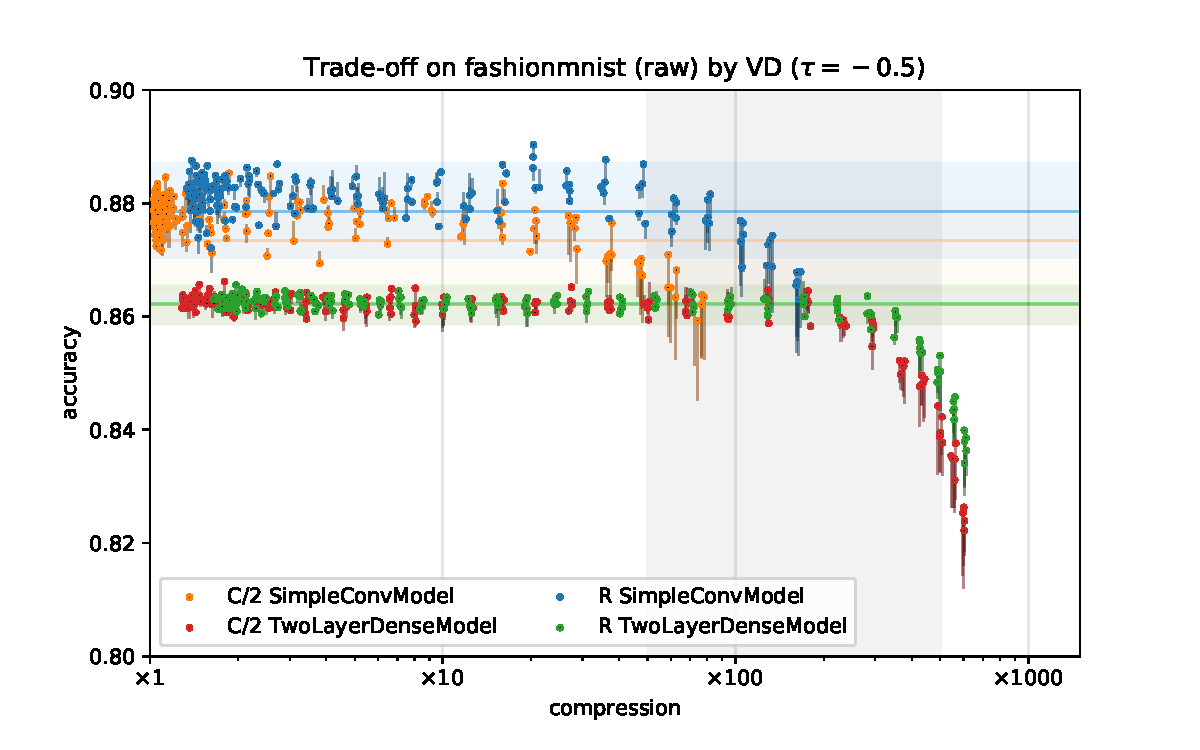
\includegraphics[width=\linewidth]{figure__mnist-like__trade-off/appendix__cmp__VD__fashionmnist__raw__-0.5.pdf}
  \end{subfigure}%
  \begin{subfigure}[b]{0.5\textwidth}
    \centering
    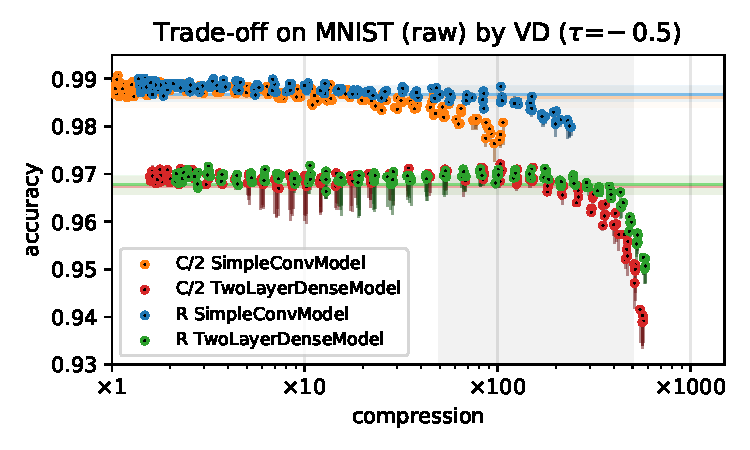
\includegraphics[width=\linewidth]{figure__mnist-like__trade-off/appendix__cmp__VD__mnist__raw__-0.5.pdf}
  \end{subfigure}
  \caption{%
    The trade-off of VD method for $\real$ and $\tfrac12\cplx$ models using raw features.
  }
  \label{fig:appendix__cmp__mnist-like__trade-off__VD__raw}
\end{figure}

\begin{figure}[b]
  \centering
  \begin{subfigure}[b]{0.5\textwidth}
    \centering
    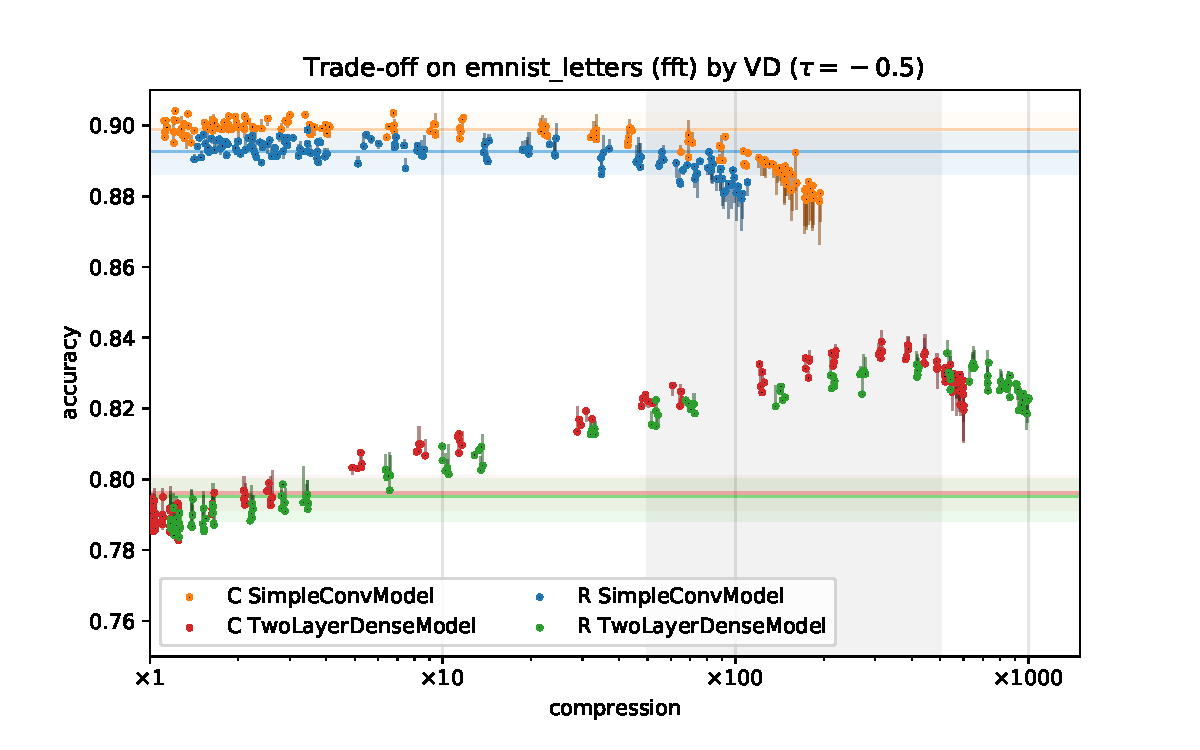
\includegraphics[width=\linewidth]{figure__mnist-like__trade-off/legacy__VD__emnist_letters__fft__-0.5.pdf}
  \end{subfigure}%
  \begin{subfigure}[b]{0.5\textwidth}
    \centering
    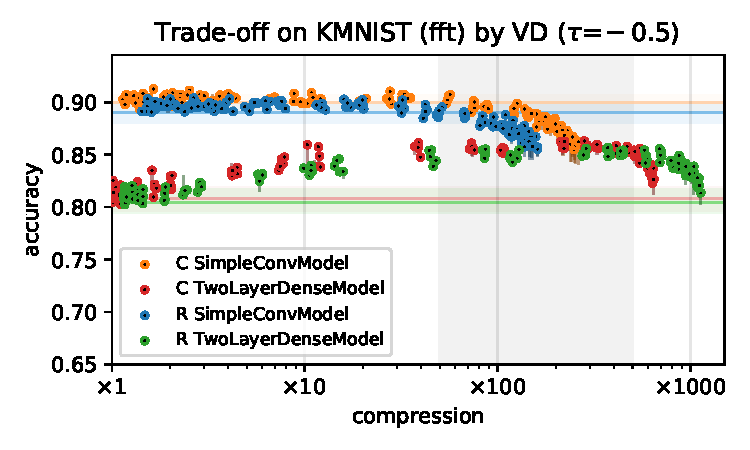
\includegraphics[width=\linewidth]{figure__mnist-like__trade-off/legacy__VD__kmnist__fft__-0.5.pdf}
  \end{subfigure} \\%
  \begin{subfigure}[b]{0.5\textwidth}
    \centering
    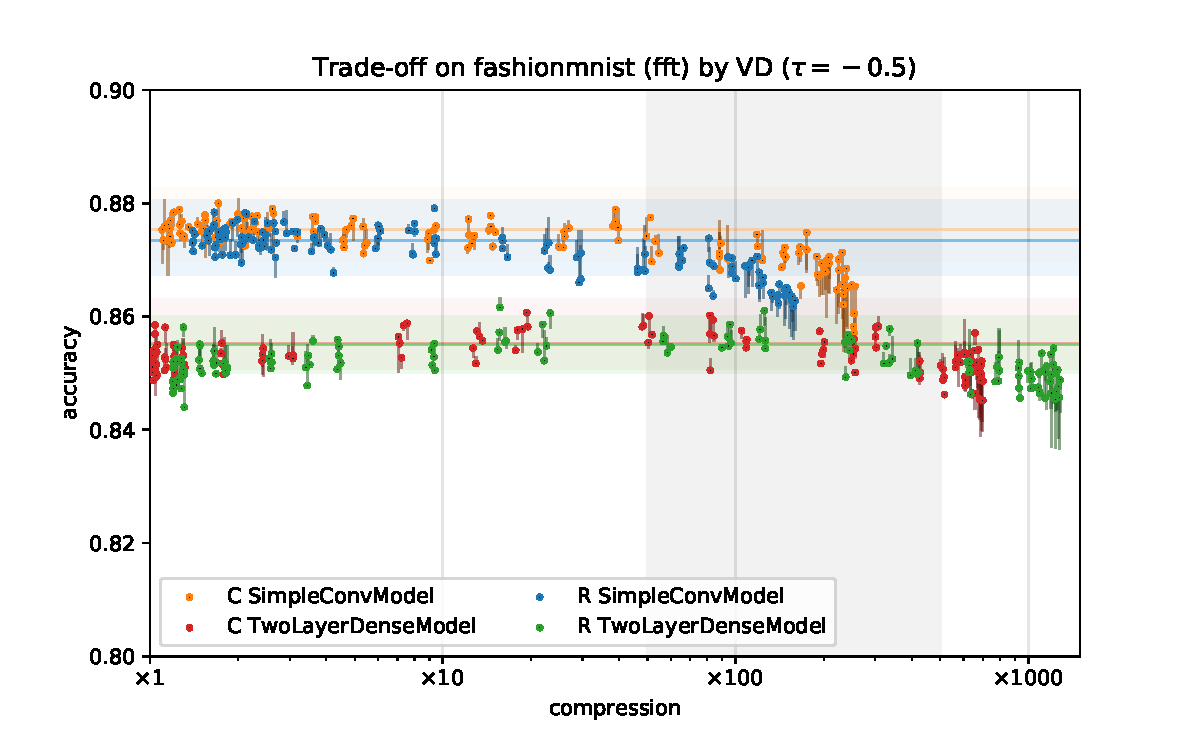
\includegraphics[width=\linewidth]{figure__mnist-like__trade-off/legacy__VD__fashionmnist__fft__-0.5.pdf}
  \end{subfigure}%
  \begin{subfigure}[b]{0.5\textwidth}
    \centering
    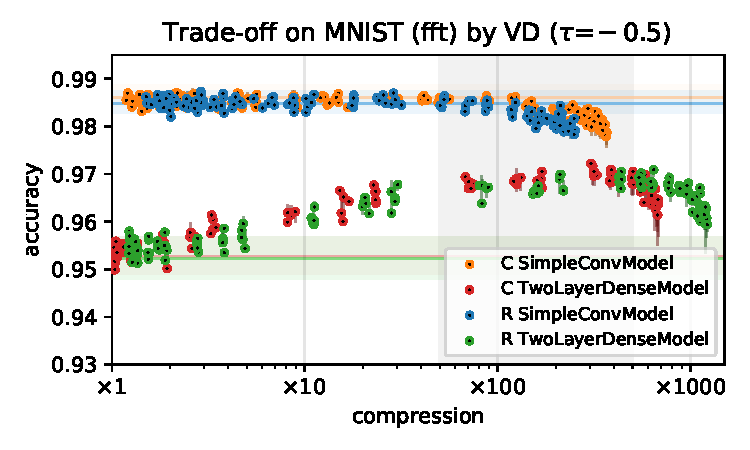
\includegraphics[width=\linewidth]{figure__mnist-like__trade-off/legacy__VD__mnist__fft__-0.5.pdf}
  \end{subfigure}
  \caption{%
    The trade-off of VD method for $\real$ and $\cplx$ models using Fourier features (main text).
  }
  \label{fig:paper__mnist-like__trade-off__VD__fft}
\end{figure}

\begin{figure}[b]
  \centering
  \begin{subfigure}[b]{0.5\textwidth}
    \centering
    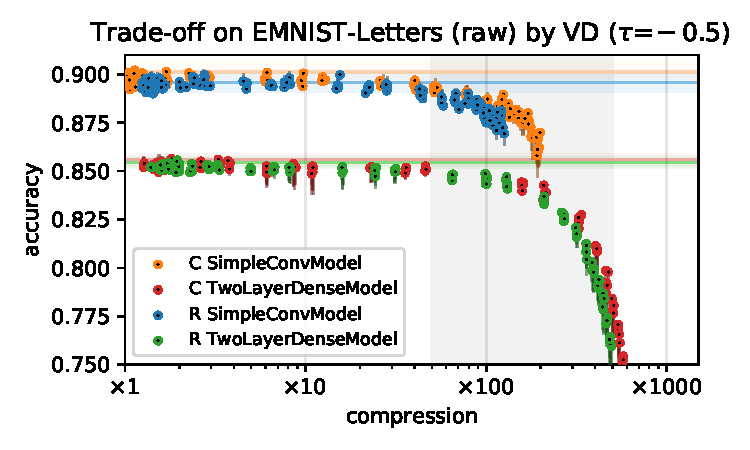
\includegraphics[width=\linewidth]{figure__mnist-like__trade-off/legacy__VD__emnist_letters__raw__-0.5.pdf}
  \end{subfigure}%
  \begin{subfigure}[b]{0.5\textwidth}
    \centering
    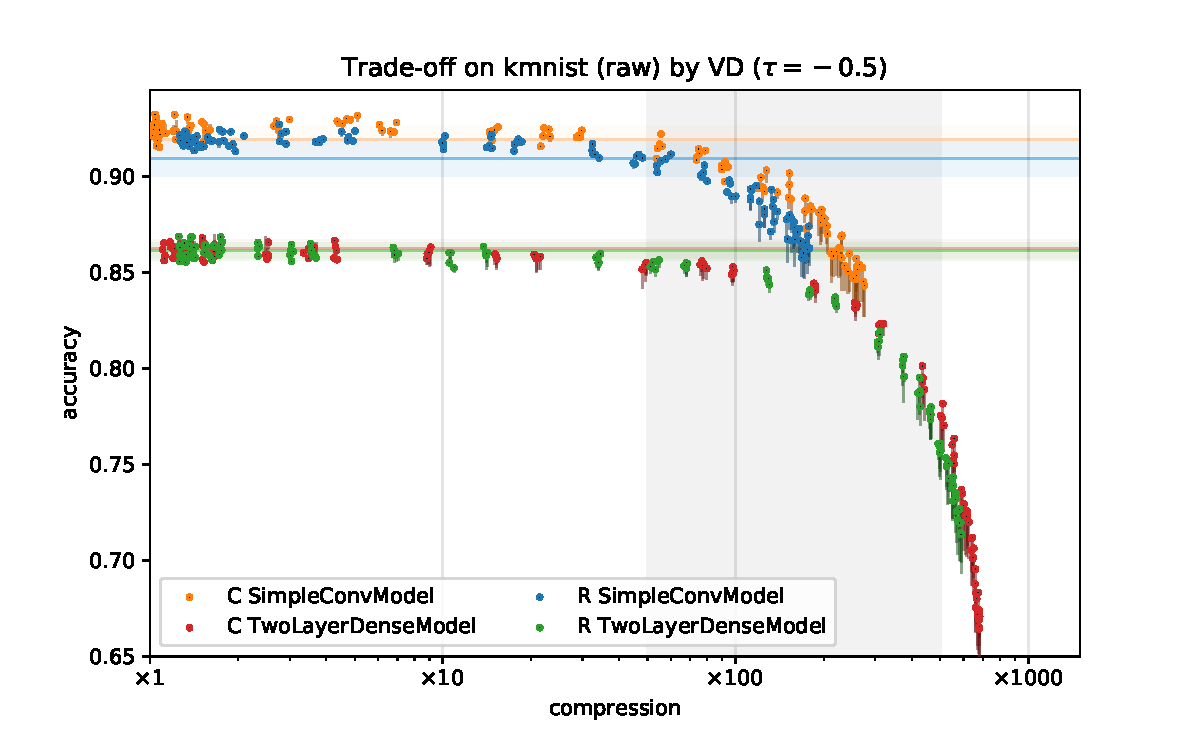
\includegraphics[width=\linewidth]{figure__mnist-like__trade-off/legacy__VD__kmnist__raw__-0.5.pdf}
  \end{subfigure} \\%
  \begin{subfigure}[b]{0.5\textwidth}
    \centering
    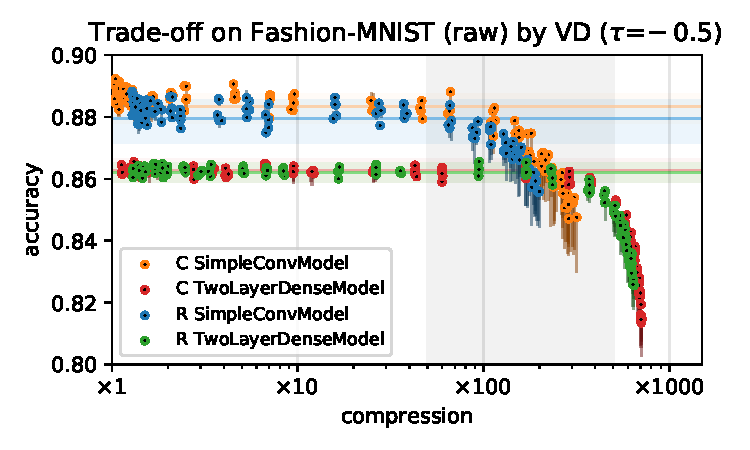
\includegraphics[width=\linewidth]{figure__mnist-like__trade-off/legacy__VD__fashionmnist__raw__-0.5.pdf}
  \end{subfigure}%
  \begin{subfigure}[b]{0.5\textwidth}
    \centering
    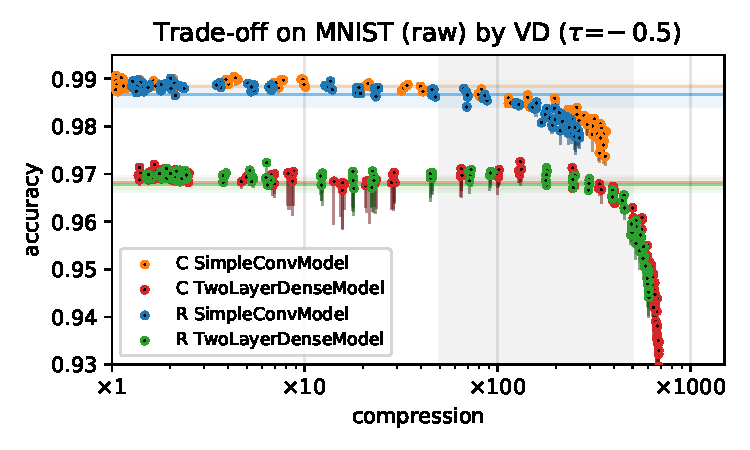
\includegraphics[width=\linewidth]{figure__mnist-like__trade-off/legacy__VD__mnist__raw__-0.5.pdf}
  \end{subfigure}
  \caption{%
    The trade-off of VD method for $\real$ and $\cplx$ models using raw features (main text).
  }
  \label{fig:paper__mnist-like__trade-off__VD__raw}
\end{figure}

% section mnist_like_experiments (end)

\clearpage

\section{CIFAR10 experiments} % (fold)
\label{sec:cifar_experiments}

In addition to the results reported in the main paper, we conduct additional experiment
on CIFAR10 and VGG16 with a much more slowly annealed learning rate. Similar to MNIST-like
experiments, we start with the rate set to $10^{-3}$ and then reduce it by $10$ after the
$10$-the epoch. In summary, for the CIFAR10 experiments we reuse the set-up with the following
changes:
\begin{itemize}
  \item we allocate $20$, $40$, and $20$ epochs to each stage
  \item the weight of the KL divergence term varies over a smaller grid $
    C \in \{
      \tfrac32 2^{-\tfrac{k}2} \colon k=7, \cdots, 15
    \}
  $
  \item we use full $50$k training split of the CIFAR10 dataset for training and raw color
  features only
  \item dataset is randomly augmented: every image within a batch of size $128$ is randomly
  cropped and flipped horizontally
\end{itemize}
Random cropping is done by zero-padding each side of a $32\times 32$ image by four pixels
and then a extracting a random $32\times 32$ patch from the $40\times 40$ intermediate image.

We experiment with $\real$ VGG16 network \citep{simonyan_very_2015} and its $\cplx$-valued
variant, which straightforwardly replaces $\real$ layers with their $\cplx$ counterparts.

\begin{figure}[htb]
  \centering
  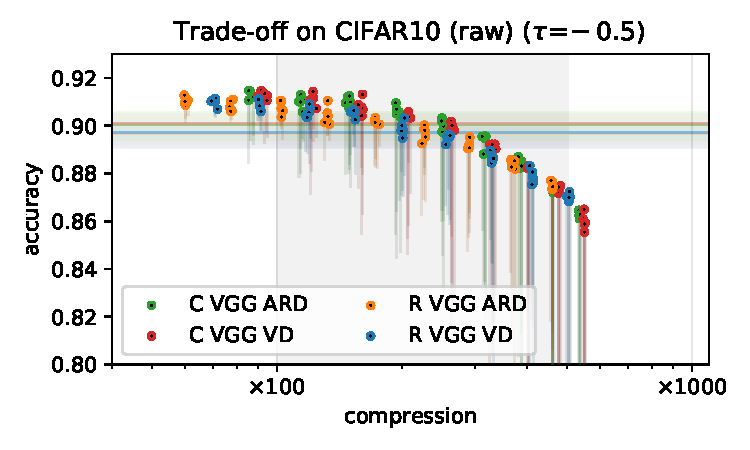
\includegraphics[width=\linewidth]{figure__cifar__trade-off/appendix__augmentedcifar10__raw__-0.5.pdf}
  \caption{%
    The compression-accuracy trade-off for $\real$ and $\cplx$ VGG16 using raw input features.
  }
  \label{fig:appendix__cifar__trade-off__VGG16__raw}
\end{figure}

% section cifar_experiments (end)

\clearpage

\bibliographystyle{abbrvnat}
\bibliography{references}

\end{document}
